% -----------------------------------------------------------------------------------------------------
% A4. Sources (final sweeps): results/A4_summary.json ((H) and (R): per-kappa geometric means and min/max over the 3
% seeds, slopes over kappa >= 10n with 95% t-intervals, K = 6; the only instances with L-SVRG and the naive schemes),
% results/A4b_summary.json ((S) and (A): slopes against the nominal kappa and against kappa_eff, over x >= 10n and over
% the window 10n <= kappa <= kappa_max, counts, kappa_eff, kappa_max), results/A4.pkl (status of the 294 runs; key
% "grid": settings selected for the naive scheme), results/A4b.pkl (seed spreads), findings.md Sec. 7. Ratios of counts,
% local slopes, seed spreads and kappa_eff/kappa are computed from these files (per-kappa geometric means over the
% seeds), and so are the fits over 10n <= kappa <= 3e4 on (H) (vrlab.analysis.loglog_slope: SAGA 1.008, L-Katyusha
% 0.510). Dimension condition on (H): q^(2m), q = (sqrt(Q)-1)/(sqrt(Q)+1), Q = 1 + 4c/mu_b, computed from the
% constants of make_hard_instance: 1.2e-10 at kappa = 3e4, 1.2e-5 at kappa = 1e5, equal to eps = 1e-8 at kappa = 4.4e4
% (findings.md Sec. 7(a); comment of experiments/exp_A4_hard_instance.py). Results referred to with \resref: A1 note,
% Props. constants, anyseq, sagamean, A4 (eq:window, eq:sagawindow, eq:lkwindow), Cor. saga, Lemma overlap, Rem. plot
% (and Sec. lb:predictions); B3 note, Prop. B3-lower; A3 note, Def. naive, Prop. naive-kappa. Factors of the two sides
% of eq:sagawindow and eq:lkwindow on (S) (7.76--7.84 and 88.6--114.9, with rho and C0 replaced by their bounds 1/105 and
% 1 + 5Q/8): Section th-A1, after Prop. A4 (6.5 for SAGA with the exact rho, Rem. plot).
% -----------------------------------------------------------------------------------------------------
\subsection{Complexity exponents on hard instances (hypothesis A4)}\label{sec:exp-A4}

\paragraph{Question and setting.}
Hypothesis A4 predicts that, for $\kappa\gg n$, the number $T$ of component gradients needed to reach
$\norm{\theta-\etastar}^2\le\varepsilon\norm{\theta_0-\etastar}^2$ grows like $\kappa$ for SAGA and like $\kappa^{1/2}$ for
L-Katyusha. On (S), \resref{prop:A4} proves $T_{\rm SAGA}=\Theta(\kappa\log\frac1\varepsilon)$ and
$T_{\rm LK}=\Theta(\sqrt{n\kappa}\log\frac1\varepsilon)$ inside the window $4n+1\le\kappa\le\kappa_{\max}(m,\varepsilon)$
of~\eqref{eq:window}, up to the constants of~\eqref{eq:sagawindow}--\eqref{eq:lkwindow} and the factor
$\log(1+\frac58Q)$ of~\eqref{eq:lkwindow}; its part (ii) gives GD and AGD the same two exponents, $L_F/\mu$ being of the
order of $Q=1+(\kappa-1)/n$ by \resref{prop:constants}. Beyond $\kappa_{\max}$ the exhaustion of the chain sets in (part
(iii) of \resref*{prop:A4}), and the counts should be read against $\kappa_{\rm eff}$, as \resref{rem:plot} explains. For $n=16$,
$m=256$ and $\varepsilon=10^{-8}$, $\kappa_{\max}\approx4.9\cdot10^4$ on (S) (the dimension term of~\eqref{eq:window}; the
slow-mode term is $1.1\cdot10^5$); on (A), a single chain of length $m=2048$, the dimension condition holds in its
sufficient form up to $(4m/\log\frac1\varepsilon)^2\approx2.0\cdot10^5$, beyond the sweep. The bounds of
Appendix~\ref{sec:lower_bound} are proved for (S), not for (H); the analogue of their dimension condition,
$q^{2m}\le\varepsilon$ with $q=(\sqrt{Q_b}-1)/(\sqrt{Q_b}+1)$ for the per-block parameter $Q_b=1+4c/\mu_b$ of (H)
(Section~\ref{sec:setting}), holds up to $\kappa\approx4.4\cdot10^4$ ($q^{2m}=1.2\cdot10^{-10}$ at $\kappa=3\cdot10^4$) and
fails at the last point of (H), $\kappa=10^5$ ($q^{2m}=1.2\cdot10^{-5}>\varepsilon$), which thus lies outside the regime in
which a span lower bound would certify the exponent $\frac12$. The counts follow the conventions of
Section~\ref{sec:exp-protocol}: for L-Katyusha the error is measured on the gradient sequence $y_t$ and $3$ gradients
are charged per iteration on average, whereas $T_{\rm LK}$ in \resref*{prop:A4} refers to the mirror sequence $z_t$ with
stored reference gradients, $2$ per iteration; the exponents are unaffected, but the measured counts of L-Katyusha are
about $\frac32$ times those of that convention, and ratios such as $T_{\rm SAGA}/T_{\rm LK}$ below are smaller by the same
factor.

On (H) and (R) the sweeps also include L-SVRG, L-Katyusha without negative momentum, and the naive scheme of
Section~\ref{sec:exp-A2}, re-tuned at every pair (instance, $\kappa$) over $\beta\in\{0.8,0.95,(\sqrt\kappa-1)/(\sqrt\kappa+1)\}$
and $\gamma R^2\in\{\frac16,\frac1{20}\}$: on (H) on seed~$0$, the choice being reused for the other seeds, and on (R),
where each seed draws a new instance, separately on each seed. Each grid run is capped at 45~s of CPU time; as the grid
runs have the same cost per iteration, a run cut by this cap had already used more gradients than the selected one
needed in total. Every run reached the target except the 30 runs of L-Katyusha without negative momentum at
$\kappa\ge10^3$, which diverge (Figures~\ref{fig:A4} and~\ref{fig:A4b}).

\begin{figure}[tbp]
  \renewcommand{\thefigure}{A4}% project figure name (see the header of this file)
  \centering
  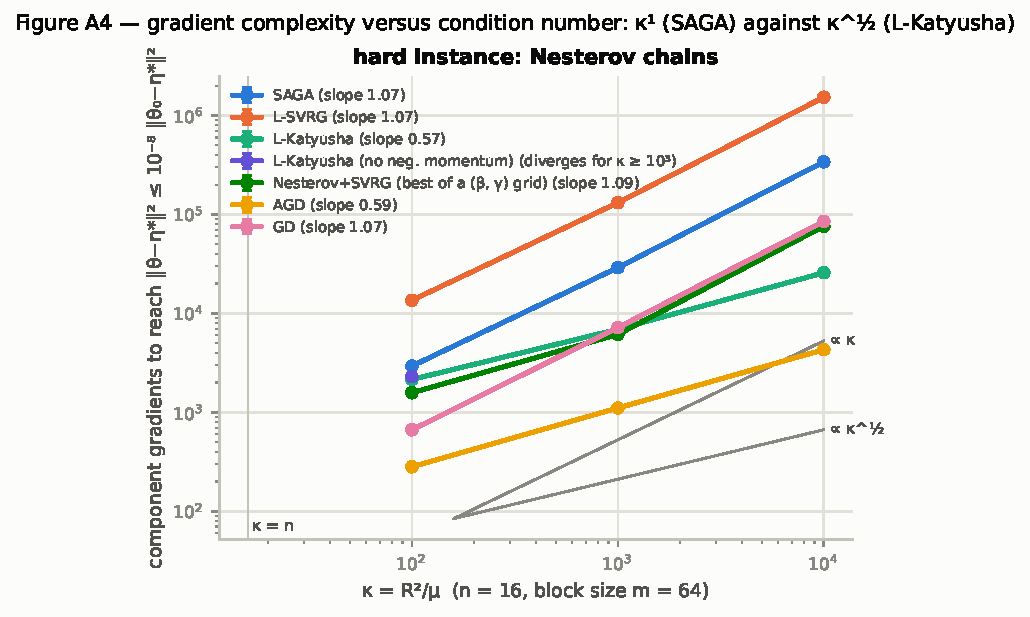
\includegraphics[width=\textwidth]{figA4_hard_instance_exponents}
  \caption{\textbf{Hypothesis A4: gradient complexity against $\kappa$.} Component gradients (counted as in
  Section~\ref{sec:exp-protocol}) needed to reach $\norm{\theta-\etastar}^2\le10^{-8}\norm{\theta_0-\etastar}^2$ (for
  L-Katyusha, $\theta=y_t$) for $\kappa\in\{10^2,3\cdot10^2,\dots,10^5\}$ ($n=16$) on (H) (block-separable Nesterov chains
  of length $m=256$, left) and on block quadratics with random spectra (R) ($m=256$, right); geometric mean over 3 seeds,
  error bars: min--max. SAGA uses $\gamma=1/(4R^2)$, L-SVRG $\gamma=1/(6R^2)$, L-Katyusha the parameters of Theorem~11
  of~\cite{kovalev2020dont}, L-Katyusha without negative momentum $\theta_2=0$ with the same $\theta_1$, $\eta$, $p$ (it
  converges only for $\kappa\in\{10^2,3\cdot10^2\}$ and diverges for every $\kappa\ge10^3$, hence no slope), the naive
  Nesterov+SVRG scheme the best of six settings
  $(\beta,\gamma R^2)\in\{0.8,0.95,(\sqrt\kappa-1)/(\sqrt\kappa+1)\}\times\{\frac16,\frac1{20}\}$, selected at each $\kappa$ on
  seed $0$ for (H) and on each seed for (R), whose instance changes with the seed, AGD and GD the step $1/L_F$. Legend:
  slope $b\pm h$, the least-squares slope of $\log(\text{gradients})$ against $\log\kappa$ fitted to the per-$\kappa$
  geometric means over the seeds, for $\kappa\ge10n$ ($K=6$), and $h$ the half-width of its $95\%$ Student interval with
  $K-2$ degrees of freedom, which measures the departure from a single power law, not sampling noise (function
  \texttt{loglog\_slope} of \texttt{vrlab/analysis.py}). Grey lines: reference slopes $1$ and $\frac12$; vertical line:
  $\kappa=n$. The only missing points are those of the divergent runs.}
  \label{fig:A4}
\end{figure}

\begin{figure}[tbp]
  \renewcommand{\thefigure}{A4b}% project figure name (see the header of this file)
  \centering
  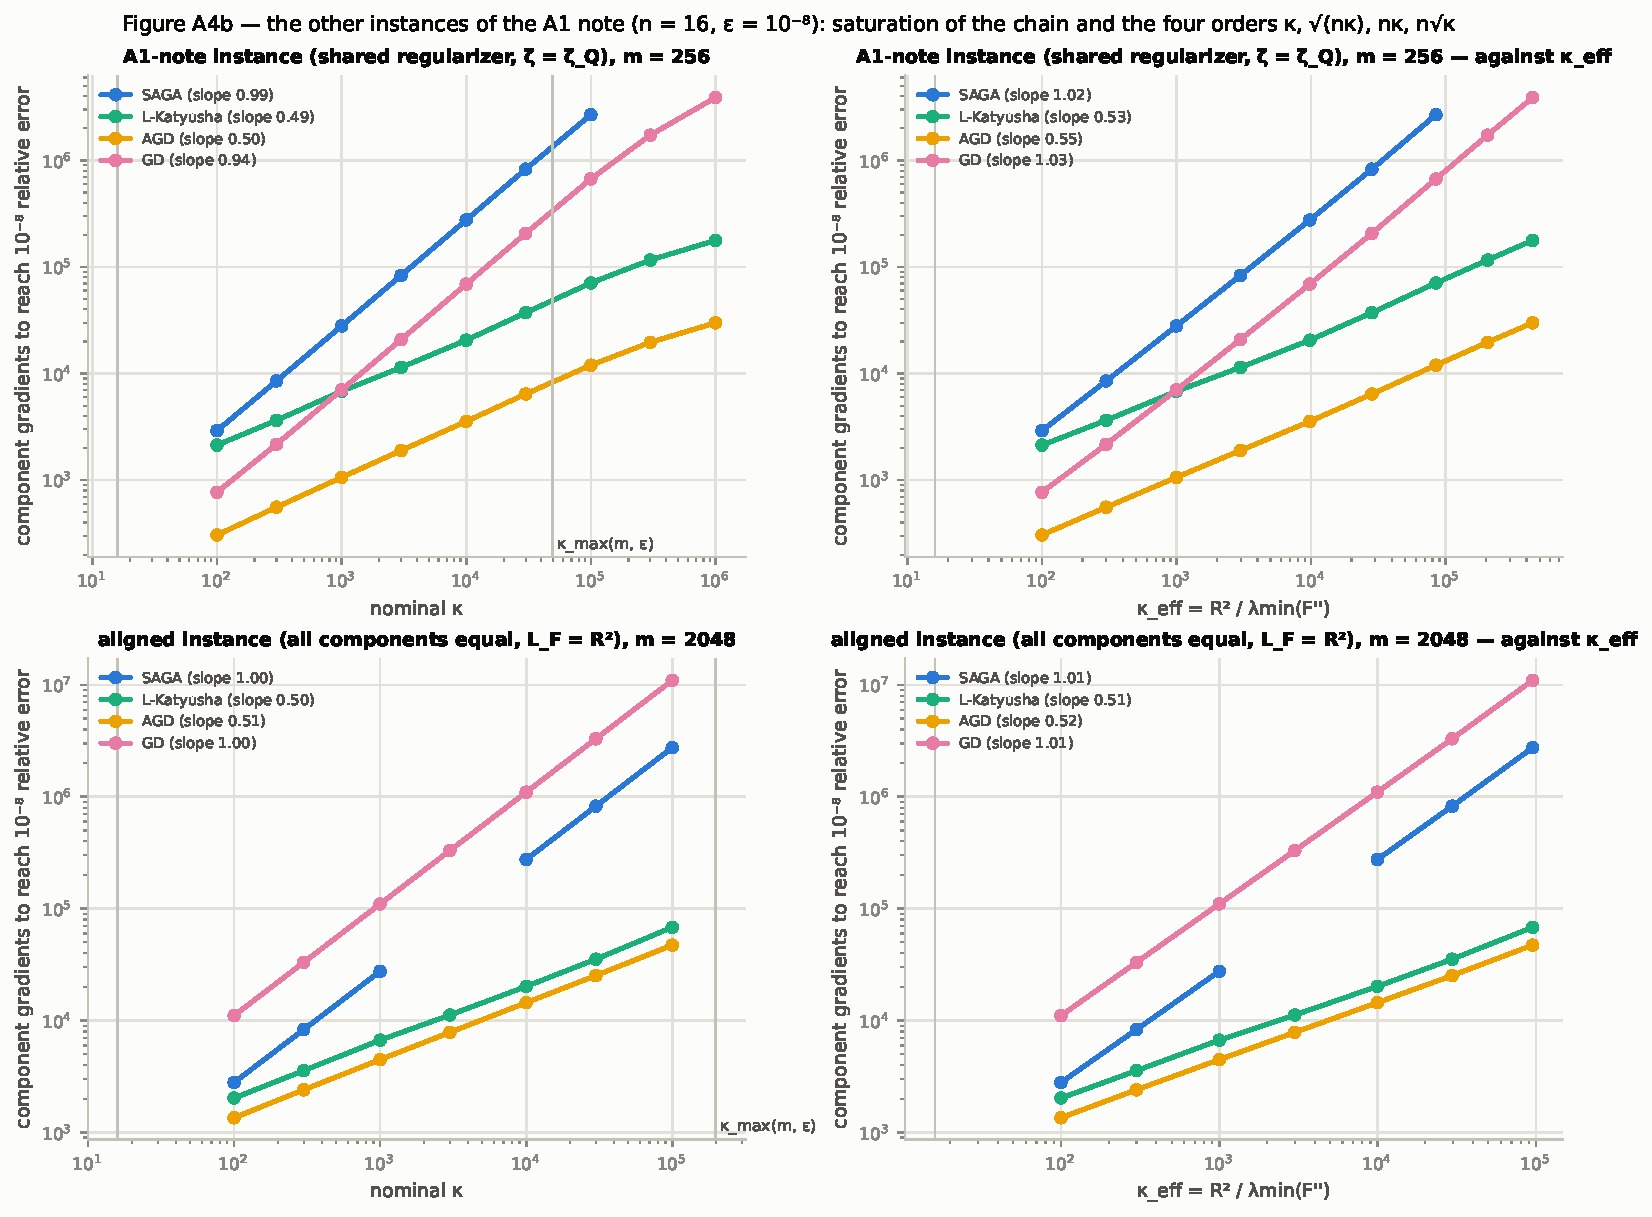
\includegraphics[width=\textwidth]{figA4b_instances}
  \caption{\textbf{Hypothesis A4 on the instances of Appendix~\ref{sec:lower_bound}.} Component gradients needed to reach
  $\norm{\theta-\etastar}^2\le10^{-8}\norm{\theta_0-\etastar}^2$ ($n=16$; geometric mean over 2 seeds; for L-Katyusha,
  $\theta=y_t$) for SAGA ($\gamma=1/(4R^2)$), L-Katyusha (parameters of Theorem~11 of~\cite{kovalev2020dont}), AGD and GD
  (step $1/L_F$), all tuned with the exact constants of the instance; L-Katyusha and AGD receive $\lmin(F'')$, not $\mu$,
  as their strong-convexity constant, so that on (S) their parameters depend on $\kappa_{\rm eff}$, not on the nominal
  $\kappa$. Top: the
  instance (S) of~\eqref{eq:instance} (shared regularizer, $\zeta=\zeta_Q$, $m=256$),
  $\kappa\in\{10^2,3\cdot10^2,\dots,10^6\}$. Bottom: the aligned instance (A) (all
  components equal to one chain of length $m=2048$, $L_F=R^2$), $\kappa\in\{10^2,3\cdot10^2,\dots,10^5\}$, on which GD and
  AGD pay the factors $n$ and $\sqrt n$ that they do not pay on (S). Left: against the nominal $\kappa$; right: against
  $\kappa_{\rm eff}=R^2/\lmin(F'')$. In the left panels the vertical line on the right marks $\kappa_{\max}(m,\varepsilon)$
  of~\eqref{eq:window} ($\approx4.9\cdot10^4$, top) and its single-chain analogue
  $(4m/\log\frac1\varepsilon)^2\approx2.0\cdot10^5$ (bottom, beyond the sweep), beyond which the chain is exhausted and the
  lower-bound argument for the exponent $\frac12$ no longer applies; in every panel the vertical line on the left marks
  $\kappa=n$. Legend: slope $b\pm h$, the least-squares slope of $\log(\text{gradients})$ against the logarithm of the
  abscissa, fitted to the per-$\kappa$ geometric means over the seeds for abscissae at least $10n$ ($K=8$ at the top, $6$
  at the bottom), and $h$ the half-width of its $95\%$ Student interval with $K-2$ degrees of freedom (function
  \texttt{loglog\_slope} of \texttt{vrlab/analysis.py}); the slopes restricted to the window
  $10n\le\kappa\le\kappa_{\max}(m,\varepsilon)$ are given in Section~\ref{sec:exp-A4}. All runs reached the target.}
  \label{fig:A4b}
\end{figure}

\paragraph{Exponents.}
The slopes $b\pm h$ of Section~\ref{sec:exp-protocol}, against $x=\kappa$ (nominal) or $x=\kappa_{\rm eff}$, are, over
$x\ge10n$ unless the window $10n\le\kappa\le\kappa_{\max}$ is indicated (the five values of the nominal $\kappa$ of (S)
from $3\cdot10^2$ to $3\cdot10^4$; L-SVRG and the naive scheme were run on (H) and (R) only):
\begin{center}
\footnotesize
\setlength{\tabcolsep}{3.5pt}
\begin{tabular}{@{}lcllllll@{}}
\toprule
instance, $x$ & $K$ & SAGA & L-SVRG & L-Katyusha & naive scheme & AGD & GD \\
\midrule
(H), $\kappa$ & 6 & $1.022\pm0.025$ & $1.021\pm0.026$ & $0.525\pm0.027$ & $0.806\pm0.188$ & $0.550\pm0.010$ & $1.026\pm0.021$ \\
(R), $\kappa$ & 6 & $1.0025\pm0.0001$ & $1.002\pm0.001$ & $0.500\pm0.005$ & $0.814\pm0.166$ & $0.526\pm0.013$ & $1.007\pm0.004$ \\
(S), $\kappa$ & 8 & $0.945\pm0.048$ & -- & $0.490\pm0.022$ & -- & $0.501\pm0.027$ & $0.944\pm0.047$ \\
(S), $\kappa$, window & 5 & $0.994\pm0.004$ & -- & $0.500\pm0.020$ & -- & $0.530\pm0.005$ & $0.990\pm0.008$ \\
(S), $\kappa_{\rm eff}$ & 8 & $1.031\pm0.017$ & -- & $0.533\pm0.019$ & -- & $0.547\pm0.007$ & $1.029\pm0.018$ \\
(S), $\kappa_{\rm eff}$, window & 5 & $1.005\pm0.015$ & -- & $0.506\pm0.025$ & -- & $0.536\pm0.009$ & $1.002\pm0.019$ \\
(A), $\kappa$ & 6 & $0.999\pm0.001$ & -- & $0.502\pm0.015$ & -- & $0.511\pm0.003$ & $0.9991\pm0.0004$ \\
(A), $\kappa_{\rm eff}$ & 6 & $1.006\pm0.008$ & -- & $0.506\pm0.018$ & -- & $0.515\pm0.006$ & $1.006\pm0.007$ \\
\bottomrule
\end{tabular}
\end{center}
On (H) and (R) the slopes are close to $1$ for SAGA, L-SVRG and GD and to $\frac12$ for L-Katyusha and AGD; the largest
deviations are those of AGD and of (H), whose local slopes rise over the last two intervals of $\kappa$ (SAGA $1.04$ and
$1.08$, L-Katyusha $0.56$ and $0.58$) and whose last point fails the analogue of the dimension condition: without this
point, the fits on (H) give $1.008$ for SAGA and $0.510$ for L-Katyusha. On (S), against the nominal $\kappa$, SAGA and
GD have the slopes $0.95$ and $0.94$, with intervals $[0.90,0.99]$ that exclude $1$: the points beyond $\kappa_{\max}$ bend
both curves (local slopes $0.98$, $0.86$ and $0.67$ between $3\cdot10^4$, $10^5$, $3\cdot10^5$ and $10^6$), whereas inside
the window their slopes are $0.994\,[0.990,0.998]$ and $0.990\,[0.982,0.998]$. On (A), where every $\kappa$ lies in the
window, they are $0.999$, against $0.50$ and $0.51$ for L-Katyusha and AGD. Several intervals exclude the predicted
exponent, by at most $0.01$ for SAGA, L-SVRG, L-Katyusha and GD on (H), on (R) and inside the windows, and by up to
$0.04$ for AGD: they measure the lack of fit of a single power law, and \resref{prop:A4} predicts the exponents only as
orders of growth, up to constant and logarithmic factors.

The naive scheme has the fitted slopes $0.81$ on both (H) and (R), with wide intervals, $[0.62,0.99]$ and $[0.65,0.98]$,
which nevertheless exclude $\frac12$; it does not follow a power law. Its best setting is the same on both instances:
$\beta=0.95$ with $\gamma R^2=\frac1{20}$ at $\kappa=10^2$, $\beta=0.95$ with $\gamma R^2=\frac16$ at
$\kappa\in\{3\cdot10^2,10^3,10^4\}$, and $\beta=(\sqrt\kappa-1)/(\sqrt\kappa+1)$ with $\gamma R^2=\frac16$ at $3\cdot10^3$ and
with $\gamma R^2=\frac1{20}$ at $\kappa\in\{3\cdot10^4,10^5\}$ (on (R) one seed selects $\beta=(\sqrt\kappa-1)/(\sqrt\kappa+1)$,
with $\gamma R^2=\frac16$, already at $\kappa=3\cdot10^2$). Its local slopes between consecutive values of $\kappa$ are
$0.82$, $0.28$, $0.73$, $1.30$, $0.79$, $0.58$
on (H) and $0.65$, $0.45$, $0.75$, $1.29$, $0.75$, $0.50$ on (R): close to $\frac12$ from $3\cdot10^2$ to $3\cdot10^3$ ($0.50$
and $0.59$; $\beta=0.95$ is the momentum $(\sqrt\kappa-1)/(\sqrt\kappa+1)$ of $\kappa\approx1.5\cdot10^3$), a jump of slope
about $1.3$ between $3\cdot10^3$ and $10^4$, then $0.5$ to $0.8$. L-Katyusha without negative momentum converges at
$\kappa=10^2$ and $3\cdot10^2$ and diverges for every $\kappa\ge10^3$ on both instances.

\paragraph{Constants, $L_F$ and finite dimension.}
On the block-separable instances the full-gradient methods share the exponents of the variance-reduced ones with
smaller constants. At $\kappa=10^5$, reaching the target costs, on (H) and (R), $1.47\cdot10^7$ and $1.49\cdot10^7$
gradients to L-SVRG, $3.27\cdot10^6$ and $3.31\cdot10^6$ to SAGA, $8.2\cdot10^5$ and $8.3\cdot10^5$ to GD, $3.1\cdot10^5$ to the
naive scheme, $7.85\cdot10^4$ to L-Katyusha and $1.3\cdot10^4$ to AGD. L-SVRG costs $4.5$ times SAGA at every
$\kappa\ge10^3$ ($4.5$--$4.6$ overall): its step $1/(6R^2)$ instead of $1/(4R^2)$ and the $3$ gradients per iteration
charged to it give $1.5\times3$ (the factor would be $3$ with stored reference gradients). The ratio
$T_{\rm GD}/T_{\rm SAGA}$ is $0.25$ on (H), (R) and (S) for every $\kappa\ge10^3$ and $4.0$ on (A) for every
$\kappa\ge10^4$; both values equal $nL_F/(4R^2)$ up to rounding, the ratio expected if the error of SAGA decays like that of
its mean iterate, which follows gradient descent with step $1/(4R^2)$ and one gradient per iteration by
\resref{prop:sagamean}, since $L_F\approx R^2/n$ on the block-separable instances and $L_F=R^2$ on (A). The counts of SAGA and of L-Katyusha agree
within $6\%$ between (S) and (A) at every common nominal $\kappa$, whereas GD costs $14$ to $16$ times more and AGD $3.9$ to
$4.4$ times more on (A): about $n$ and $\sqrt n$, the factors by which $nL_F/\mu$ and $n\sqrt{L_F/\mu}$ grow when $L_F$ goes
from about $R^2/n$ to $R^2$. The ratio $T_{\rm SAGA}/T_{\rm LK}$ grows like $\sqrt{\kappa/n}$, with a constant between $0.52$
and $0.54$ over the whole sweep on (H) and (R) ($41.7$ and $42.1$ at $\kappa=10^5$, where $\sqrt{\kappa/n}=79$), between
$0.51$ and $0.55$ on (A), and of $0.54$ and $0.48$ at $\kappa=10^4$ and $10^5$ on (S) ($13$ and $38$); with the counting
convention of \resref{prop:A4}, which stores the reference gradients, these constants would be about $\frac32$ times
larger. On (S), $\kappa_{\rm eff}/\kappa$ is $0.98$ at the nominal $\kappa=10^4$, $0.85$ at $10^5$ and $0.44$ at $10^6$; the
slopes of SAGA and GD drop from $0.99$ inside the window to $0.95$ and $0.94$ over $\kappa\ge10n$ against the nominal
$\kappa$, and are both $1.03$ against $\kappa_{\rm eff}$: plotting against $\kappa_{\rm eff}$ largely removes the bend, as
part (iii) of \resref*{prop:A4} and \resref{rem:plot} anticipate, with a slight overshoot (local slopes against
$\kappa_{\rm eff}$ up to $1.07$ between $3\cdot10^4$ and $3\cdot10^5$). L-Katyusha and AGD, whose parameters depend on
$\lmin(F'')$, i.e.\ on $\kappa_{\rm eff}$, rather than on $\mu$, bend less ($0.50$ to $0.49$ and $0.53$ to $0.50$), and
their slopes against $\kappa_{\rm eff}$, $0.53$ and $0.55$, are slightly above $\frac12$. The theory does not fix these
values: inside the window its bounds leave constant and logarithmic factors, such as the $\log(1+\frac58Q)$
of~\eqref{eq:lkwindow}, and beyond $\kappa_{\max}$ the lower bound behind the exponent $\frac12$ no longer applies, while
the upper bounds involve $\lmin(F'')$ rather than $\mu$ because of this tuning (for L-Katyusha, part (iii) of
\resref*{prop:A4}, with $\kappa_{\rm eff}$ in place of $\kappa$).

\paragraph{Interpretation.}
The exponents predicted by hypothesis A4 are observed on the four instances with 2 or 3 seeds, up to the constant and
logarithmic factors of \resref{prop:A4}: over $\kappa\ge10n$ and against the nominal $\kappa$, the slopes are $0.95$--$1.02$
for SAGA ($0.95$ on (S), whose chain is exhausted beyond $\kappa_{\max}$; $0.99$ inside its window and $1.03$ against
$\kappa_{\rm eff}$), $1.00$--$1.02$ for L-SVRG (on (H) and (R), the two instances where it was run) and $0.49$--$0.52$ for
L-Katyusha. As orders of growth, the exponent $1$ of SAGA is a theorem for constant steps, by \resref{prop:B3-lower},
and, on (S) and (A), inside their windows and for the step $1/(4R^2)$ of the experiments, by \resref{cor:saga} with
\resref{lem:overlap}; on (S) the exponent $\frac12$ of L-Katyusha is optimal inside the window, by \resref{prop:anyseq}
with part (ii) of \resref*{prop:A4}. The measured slopes agree with these orders, which do not by themselves fix the
value of a slope fitted over a finite window: the two sides of~\eqref{eq:sagawindow} and of~\eqref{eq:lkwindow}, with
$\rho$ and $C_0$ replaced by their bounds, differ there by factors of about $8$ and $10^2$ (Section~\ref{sec:th-A1} and
\resref*{rem:plot}).
The expectation of the proposal that AGD costs $n\sqrt\kappa$ and GD $n\kappa$ holds only when $L_F\approx R^2$, as on
(A): on block-separable instances, the worst case for incremental methods, the full-gradient methods do at least as well
as their variance-reduced counterparts, and what variance reduction buys is the uniform guarantee over all instances with
given $(n,R^2,\mu)$ (Section~\ref{sec:lb:predictions}). The re-tuned naive scheme, a variant of the scheme
of \resref{def:naive} (Section~\ref{sec:exp-A2}), has fitted slopes between the two exponents on this grid. This is
consistent with, but not predicted by, the obstruction that \resref{prop:naive-kappa} proves for the scheme
of \resref*{def:naive} itself, a limit of the proof, and with the absence of an acceleration guarantee for such schemes
with one sample per iteration~\cite{nitanda2014stochastic}; it does not show that no tuning can accelerate the scheme.
